\documentclass[11pt,letterpaper,leqno]{amsart}
\usepackage[latin1]{inputenc}  % Unixin merkist�
\usepackage[T1]{fontenc}       % kirjaimet, joissa aksentteja (skandit)


\usepackage{amsfonts}         
\usepackage{amsmath}
\usepackage{amssymb}
\usepackage{amsthm}
\usepackage{ae,aecompl,amsbsy}
\usepackage{epsf}
\usepackage{graphics}
\usepackage{ucs}
\usepackage[pdftex]{graphicx}
\usepackage{amsaddr}
%\usepackage[foot]{amsaddr}


\usepackage{color}
\usepackage{verbatim}
\usepackage{algorithm}
\usepackage{algorithmic}
\usepackage{caption}
\usepackage{subcaption}


\newcommand{\R}{\mathbb{R}}
\newcommand{\C}{\mathbb{C}}
\newcommand{\Q}{\mathbb{Q}}
\newcommand{\N}{\mathbb{N}}
\newcommand{\Z}{\mathbb{Z}}

\newcommand{\divergence}{\operatorname{div}}
\DeclareMathOperator*\argmin{argmin}

\newcommand{\TODO}[1]{\textcolor{red}{{\sc Todo:} #1}}
% Lauseet, m��ritelm�t ja esimerkit


\newtheorem{definition}[equation]{Definition}
\newtheorem{proposition}[equation]{Proposition}
\newtheorem{assumption}[equation]{Assumption}
\usepackage{lineno}


\numberwithin{equation}{section}
\graphicspath{ {figures/} }

\title{Analytical results and physical understanding}
\author{Team C}
%\address{Math 512}
%\date{\today}     
%\email{sannatyr@math.ubc.ca}
                               
\begin{document}
%\linenumbers
\maketitle
\thispagestyle{empty}

\Large
\textbf{Uniform electric field illuminating a sphere in a uniform earth (analytic solution, reference)}

\vspace{0.4cm}

Let consider a  resistive uniform half-space, of conductivity $\sigma_1$enclosing a conductive sphere $\sigma_2$. Let assume a uniform, unidirectional static electric field $E_0$ going through this half-space.

\begin{figure}[h]
\caption{Uniform electric field illuminating a sphere in a uniform earth}
\includegraphics[scale=0.7]{electrostaticsphere.png}
\end{figure}

\vspace{0.4cm}
\textbf{Maxwell equations}
\vspace{0.4cm}


In this case, we need:

 \vspace{0.4cm}


$\nabla \times E =0$ \quad,so \quad $E=-\nabla V$	\quad	(1)

\vspace{0.4cm}

$J=\sigma E$ \quad (2)


\vspace{0.4cm}



The primary field $E_0$ can then be expressed by:

\vspace{0.4cm}

${E^p}_0=-\frac{dV^p}{dx}$ \quad (3)
\vspace{0.4cm}
Assuming a primary potential null at the origin:

 \vspace{0.4cm}


$V^p=E_0x=E_0 r cos\theta$ \quad (4)

 \vspace{0.4cm}



As the primary potential respects $\nabla^2 V=0 $, as only a dependence in $x$ direction, the anomalous or secondary field can be expressed as (using spherical coordinates):

 \vspace{0.4cm}


$V^s=(A r + B r^{-2}) cos\theta$ \quad (5)


\vspace{0.4cm}

If we assume finite  values of the potential everywhere, we can divide the anomalous potential in two domain:

 \vspace{0.4cm}


${V^s}_e=B r^{-2} cos\theta$ \quad if $r>R$ \quad (6)

 \vspace{0.4cm}


${V^s}_i=A r cos\theta$ \quad if $r<R$ \quad (7)

 \vspace{0.4cm}



The total external potential is then:

 \vspace{0.4cm}


$V_e= {V^s}_e + {V^p} = (-E_0 r + B r^{-2}) cos \theta$ \quad (8)


 \vspace{0.4cm}


On the surface of the sphere, both the normal current density and potential have to be continuous across the interface.

 \vspace{0.4cm}


Using the continuity of current density, we got:
$\sigma_1 E_e = \sigma_2 E_i$ \quad $\sigma_1 \frac{dV_e}{dr} = \sigma_2 \frac{dV_e}{dr} $ \quad (9)

 \vspace{0.4cm}



$2 \sigma_1 B R^{-3} + \sigma_1 E_0$ \quad (10)


 \vspace{0.4cm}


Using the continuity of potential, we got:

 \vspace{0.4cm}


${V_e}={V^s}_i$	\quad (11)

 \vspace{0.4cm}


$-E_0 R + B R^{-2} = A R$ \quad (12)

 \vspace{0.4cm}


From equations (10) and (12), we get:

 \vspace{0.4cm}


$A=-\frac{3 \sigma_1}{\sigma_2 + 2\sigma_1} E_0 $ \quad (13)

 \vspace{0.4cm}


$B=E_0 R^3 \frac{\sigma_2-\sigma1}{\sigma_2+2\sigma_1} $ \quad (14)

 \vspace{0.4cm}


And the anomalous electric field is:

 \vspace{0.4cm}


$\mathbf{E_s=-\nabla{V^s}_e=E_0 R^3 \frac{\sigma_2-\sigma_1}{\sigma_2 - 2\sigma_1} \frac{(2x^2-y^2-z^2)\mathbf{u}_x + 3xy \mathbf{u}_y + 3xz \mathbf{u}_z}{r^5}} $ \quad (15)

\vspace{0.4cm}


\Large
\textbf{Continuity of current and charge accumulation}

\vspace{0.4cm}

We assume to be here in a steady state with direct current.
The current entering a cylinder through an interface as in figure \ref{Normal J continuous} consists both in tangential and normal components. 

\begin{figure}[h]
\caption{Uniform electric field illuminating a sphere in a uniform earth}
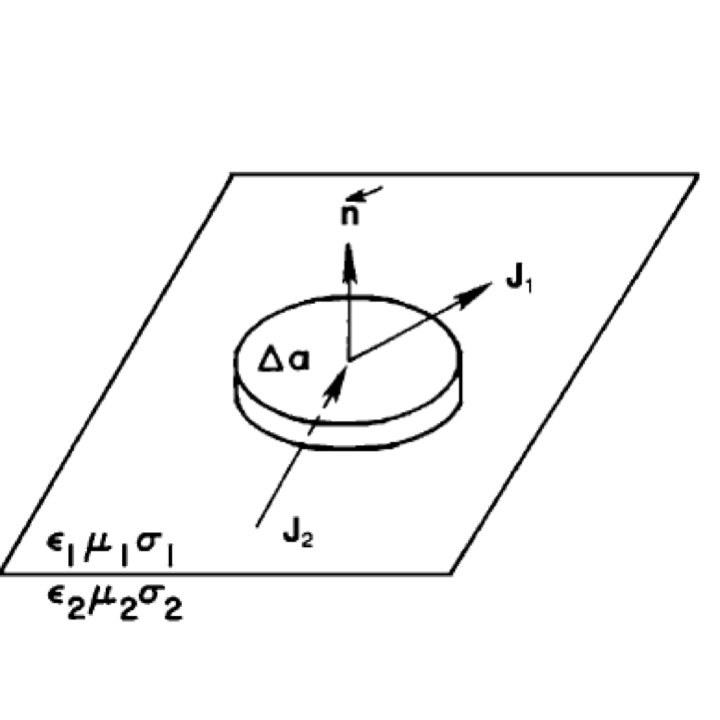
\includegraphics[scale=0.2]{Jcontinuous.png}
\label{Normal J continuous}
\end{figure}

As the cylinder height is collapsed to zero, we can write the normal component as:

$I=J_1 \cdot \mathbf{n} \Delta a$ \quad (16)
or as
$I=J_2 \cdot \mathbf{n} \Delta a$ \quad (17)
\vspace{0.4cm}

Note: Otherwise in steady state we would have an infinite built up of charges at the interface 
\vspace{0.4cm}
Then $J_2 \cdot \mathbf{n} = J_1 \cdot \mathbf{n}$ \quad (18)
\vspace{0.4cm}

so $\mathbf{{J_1}^n={J_2}^n}$ \quad (19)

\vspace{0.4cm}
Note: This is only true in a direct current case in a steady state. It appears to be satisfactory up to $10^5$ Hz, as long as displacement currents can be considered negligeable.

\vspace{0.4cm}

\Large
\textbf{Charges, Coulomb's law and potentials.}

Electric charge produces an electric potential; the Coulomb's electrostatic potential is

%\begin{equation}
$V(r) = \frac{1}{4\pi\epsilon_0}\frac{Q}{r}.$ \quad (20)
%\end{equation}

 \vspace{0.4cm}



\Large
\textbf{Anomalous currents and electric fields}

Anomalous current density is defined as 
%\begin{equation*}
$\mathbf{J}_a = \sigma_a\mathbf{E}.$ \quad (21)
%\end{equation*}


Here $\mathbf{E}$ is total electric field and $\sigma_a$ is the difference between wholespace conductivity $\sigma_1$ and conductivity of the target $\sigma_2$: $\sigma_a = \sigma_2-\sigma_1$.



 \vspace{0.4cm}



DC app for looking at currents, charges etc with a current source at the surface.


 \vspace{0.4cm}



\Large
\textbf{Analytic solution for a buried sphere in a uniform space}


\end{document}